% asset_id: FAS2EulerianTraversabilityAndRouteInspectionTikZ-003
% asset_type: TikZ
% unit_code: FAS2
% topic_code: FAS2-GRAPH
% topic_id: FAS2EulerianTraversabilityAndRouteInspection
\documentclass[tikz,border=8pt]{standalone}
\usetikzlibrary{positioning,calc}
\begin{document}
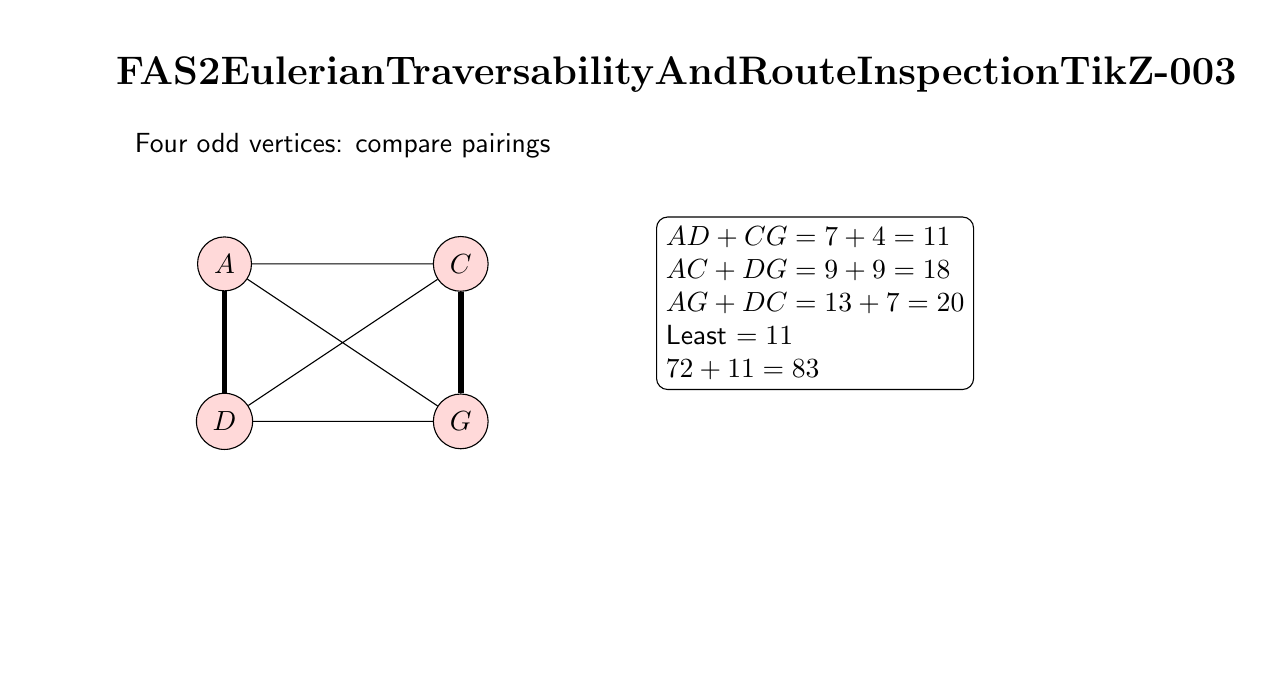
\begin{tikzpicture}[font=\sffamily]
\fill[white] (-1,-1) rectangle (13,7);
\node[anchor=west,font=\bfseries\Large] at (0,6.4) {FAS2EulerianTraversabilityAndRouteInspectionTikZ-003};

\node at (3,5.5) {Four odd vertices: compare pairings};
\node[circle,draw,fill=red!15] (A) at (1.5,4) {$A$};
\node[circle,draw,fill=red!15] (C) at (4.5,4) {$C$};
\node[circle,draw,fill=red!15] (D) at (1.5,2) {$D$};
\node[circle,draw,fill=red!15] (G) at (4.5,2) {$G$};
\draw (A)--(C)--(G)--(D)--cycle (A)--(G) (C)--(D);
\draw[line width=2pt] (A)--(D) (C)--(G);
\node[draw,rounded corners,align=left] at (9,3.5) {$AD+CG=7+4=11$\\$AC+DG=9+9=18$\\$AG+DC=13+7=20$\\Least $=11$\\$72+11=83$};

\end{tikzpicture}
\end{document}
